\chapter{Aplicaciones}

\section{Minimización del máximo autovalor}

\noindent Referencia principal: \cite[Sección 3, Ejemplo 1]{Todd2001}.

Este problema aparece por ejemplo en la estabilización de ecuaciones diferenciales.

Suponemos que tenemos una matriz simétrica $M(z)$ que depende linealmente (afín) de un vector $z$. Queremos elegir $z$ que minimice el máximo autovalor de $M(z)$. Observemos que
$$
\lambda_{\max}(M(z)) \le \eta \text{ si y solo si } \lambda_{\max}(M(z) - \eta I) \le 0,
$$
o equivalentemente, $\lambda_{\min}(\eta I - M(z)) \ge 0$. Esto se cumple si y solo si $\eta I - M(z) \succeq 0$. Obtenemos entonces el problema SDP en forma dual:
\begin{alignat*}{2}
  & \text{maximizar: } & & -\eta \\
   & \text{sujeto a: } & \quad & \eta I - M(z) \succeq 0.
\end{alignat*}

El problema contrario, maximizar el mínimo autovalor puede interpretarse como obtener la matriz ``lo más positiva posible''. Veremos más adelante cómo utilizar este problema SDP para calcular descomposiciones en suma de cuadrados de polinomios.


\section{Optimizaci\'on combinatoria: maxcut}

\noindent Referencias principales: \cite[Sección 3, Ejemplo 9]{Todd2001}, \cite[Lección 14]{ODonell2008}.

Comenzamos con un grafo no-dirigido $G = (V, E)$, donde $V$ es el conjunto $\{v_1, \dots, v_n\}$ de $n$ nodos y $E \subset V \times V$ es el conjunto de aristas.
Definimos una matriz de costos no-negativos $W = (w_{ij}) \subset \R_{\ge 0}^{n \times n}$. Podemos suponer que el grafo es completo, es decir que todos los nodos son adyacentes entre sí, tomando $w_{ij} = 0$ para todas las no-aristas $ij$; definimos también $w_{ii} = 0$ para todo $i$. $W$ resulta una matriz simétrica.

Para un subconjunto $K \subset N$ de nodos, definimos el corte $\delta(K)$ como el conjunto de todos las aristas desde $K$ al complemento de $K$:
$$
\delta(K) = \{(i,j) \in E : i \in K, j \notin K\}.
$$
Dado un corte $K$ definimos el costo del corte
$$
w(\delta(K)) := \sum_{(i,j) \in \delta(K)} w_{ij}.
$$
Queremos hallar el corte con el mayor costo posible.

\begin{example}
En el siguiente grafo de 5 nodos, asignamos costo 1 a todas las aristas dibujadas y costo 0 a las aristas no dibujadas. Tomando $K$ el conjunto de nodos blancos, obtenemos el corte de mayor costo posible.
\begin{center}
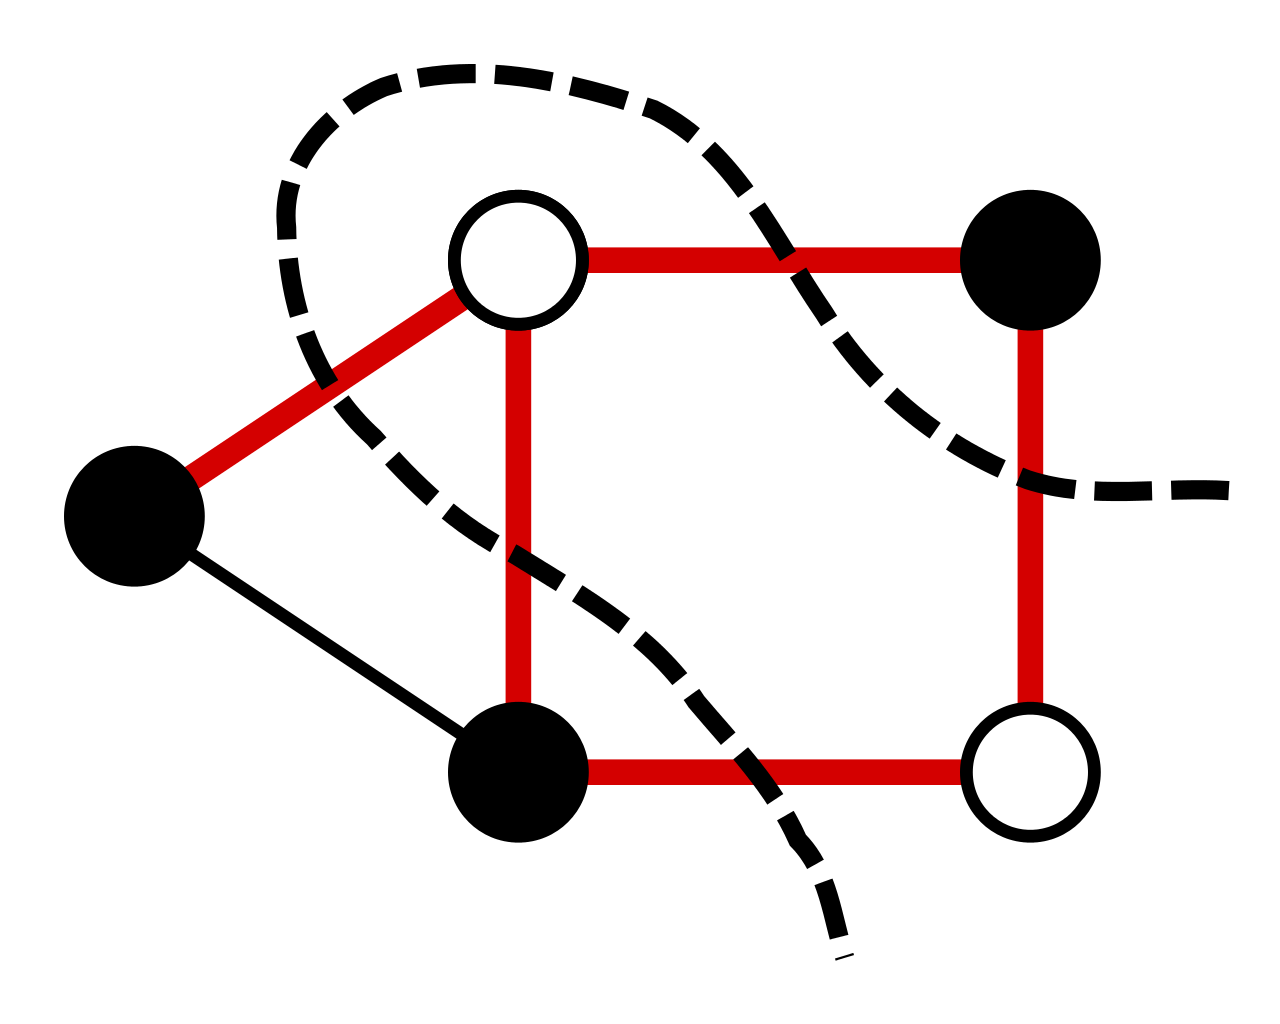
\includegraphics[scale=.2]{1280px-Max-cut.png}
\end{center}
\end{example}


\begin{example}
Si consideramos un grafo completo de 4 vértices, con costo 1 en todas las aristas, el costo de un corte queda determinado por la cantidad de nodos en el corte. Obtenemos los siguientes valores:
$$
\delta(K) = \begin{cases}
0 & \text{ si } \#K = 0, \\
3 & \text{ si } \#K = 1, \\
4 & \text{ si } \#K = 2, \\
3 & \text{ si } \#K = 3, \\
0 & \text{ si } \#K = 4. \\
\end{cases}
$$

Por lo tanto, para obtener el corte de mayor costo tomamos un conjunto $K$ de 2 elementos.
\end{example}



Comenzamos formulando el problema en forma matricial. Queremos calcular el costo de un corte mediante un producto de matrices. Fijamos un corte $K$ y definimos el vector $\xb = (\xb_1, \dots, \xb_n) \in \R^n$ por
$$
x_i = \begin{cases}
1 & \text{ si } v_i \in K \\
-1 &  \text{ si } v_i \notin K
\end{cases}.
$$
De esta forma, $x_i x_j = -1$ si $(i,j) \in \delta(K)$ y $x_i x_j = 1$ si $(i,j) \notin \delta(K)$, y por lo tanto
$$
1 - x_i x_j = \begin{cases}
0 & \text{ si } (i,j) \in \delta(K) \\
2 &  \text{ si } (i,j) \notin \delta(K).
\end{cases}
$$
Obtenemos
$$
w(\delta(K)) = \frac{1}{2}\sum_{i < j}w_{ij}(1-x_i x_j) = \frac{1}{4}\sum_{i \neq j}w_{ij}(1-x_i x_j).
$$
Como además $w_{ii} = 0$ para todo $i$,
$$
w(\delta(K)) = \frac{1}{4}\sum_i \sum_j w_{ij}(1-x_i x_j) = \left(\frac{1}{4}\sum_i \sum_j w_{ij} \right) - \frac{1}{4} x^T W x.
$$

Para poder juntar los últimos dos términos en uno, reescribimos:
$$
\left(\frac{1}{4}\sum_i \sum_j w_{ij} \right) - \frac{1}{4} x^T W x = \left(\frac{1}{4}\sum_i \left(\sum_j w_{ij}\right) x_i x_i \right) - \frac{1}{4} x^T W x.
$$
y definiendo $C \in \R^{n \times n}$ con $c_{ij} = -w_{ij}/4$ para $i \neq j$ y $c_{ii} = \sum_j w_{ij}/4$ para todo $i$ obtenemos
$$
w(\delta(K)) = x^T C x.
$$

Finalmente, como cualquier vector $x \in \{-1, 1\}^n$ define un corte, podemos escribir el problema max-cut como el problema de programación cuadrática entera:
$$
\text{(IQP):} \quad \max x^TCx, x_i \in \{+1, -1\}, i \in N,
$$
o como un problema cuadrático con restricciones cuadráticas no-convexas
$$
\text{(NQCQP):} \quad \max x^TCx, x_i^2 = 1, i \in N.
$$

Ninguna de estas dos formulaciones corresponde a un problema de programación semidefinida. A continuación veremos como relajar las condiciones para obtener un problema SDP.

\subsection{Relajación 1}
Observamos que (NQCQP) es linear en los productos $x_i x_j$ y que estos productos son las coordenadas de la matriz $X = xx^T \in \R^{n \times n}$ de rango 1. Más aún, $X$ es simétrica, $X_{ii} = 1$ para todo $i$ y $X \succeq 0$. Recíprocamente, cualquier matriz de rango 1 con esas propiedades puede escribirse como $xx^T$ para algún vector $x \in \{-1, 1\}^n$. (COMPLETAR DEMOSTRACION: $X = y x^T$, y podemos tomar $y = x$ y como $x_i^2 = 1$ es de la forma buscada.)

Finalmente, como $x^T C x = C \bullet (xx^T)$, obtenemos que (IQP) es equivalente al problema
$$
\max C \bullet X, \quad X_{ii} = 1, i \in N, X \succeq 0, \rank(X) = 1.
$$

Eliminando la restricción del rango, obtenemos el problema SDP
$$
\max C \bullet X, \quad X_{ii} = 1, i \in N, X \succeq 0.
$$

\subsection{Relajación 2}

Observemos que en (IQP) asociamos a cada nodo $v_i$ un valor $x_i \in \{-1, 1\}$, que podemos considerar como un vector unitario de dimensión 1.
Ahora, en cambio, asociamos a cada nodo $v_i$ un vector unitario $p_i \in \R^n$, y consideramos la matrix $\Pb$ con estos vectores como filas. Reemplazamos entonces la función objetivo $C\bullet (xx^T)$ por $C \bullet (PP^T)$ y las restricciones $x_i \in \{+1, -1\}$ por restricciones de los elementos de la diagonal de $PP^T$: $(PP^T)_{ii} = 1$. Como $PP^T$ es  semidefinida positiva, y cualquier matrix semidefinida positiva se puede factorizar de esta forma, vemos que mediante esta construcción obtenemos el mismo problema SDP de antes.
Considerando una matriz $\Pb$ donde todas las filas son de la forma $v$ o $-v$ para un vector unitario $v$, vemos que este problema es efectivamente una relajación del problema (IQP).

\subsection{Relación entre la relajación y el problema original}

Como las formulaciones SDP son relajaciones del problema max-cut, el valor óptimo del problema SDP es una cota superior del valor óptimo del problema original. Pero vamos a ver que podemos usar la solución del problema SDP para obtener un corte razonablemente bueno.

Usamos la segunda relajación, y tomamos $X = PP^T$ una solución óptima de ese problema. Si todas las filas de $\Pb$ fueran $+v$ o $-v$ para un vector $v$, definimos el corte tomando en $K$ todos los nodos para los cuales la fila correspondiente es $+v$.

En la situación general, tomamos un hiperplano que divide a la esfera unitaria en dos mitades y tomamos en $K$ a todos los nodos que quedan en una de estas dos mitades.

Más concretamente, para un vector aleatorio $g$ de norma 1, definimos
$$
K = \{v_i \in V: g^T p_i \ge 0\}.
$$

Esto nos da un corte aleatorio, y podemos calcular la esperanza  del valor del corte (veremos más adelante cómo tomar un vector aleatorio).

La esperanza del valor del corte es
$$
E[w(\delta(K))] = E\left[\sum_{i,j} w_{ij} \one_{(i,j) \in \delta(K)}\right] = \sum_{i,j} w_{ij} \Pr[(i,j) \in \delta(K)].
$$
(observamos que las probabilidades no son independientes, pero no es necesaria independencia para distribuir la esperanza con respecto a la suma).

Calculamos ahora $\Pr[(i,j) \in \delta(K)]$ para $(i,j)$ fijo. Consideramos el plano que pasa por el origen y contiene a los dos vectores $p_i$ y $p_j$. La probabilidad de que un hiperplano separe a los dos vectores es la misma que la probabilidad de que un diámetro en este plano los separe. Esta probabilidad es
$$
GW(K) = \Pr[(i,j) \in \delta(K)] = \frac{\angle(p_i, p_j)}{\pi} = \frac{\arccos(p_i \cdot p_j)}{\pi}.
$$

Por lo tanto, el valor esperado del corte es
$$
E[w(\delta(K))] = \sum_{i,j} w_{ij} \frac{\arccos(p_i \cdot p_j)}{\pi}
$$
y queremos comparar este valor
$$
SDP(K) = \sum_{i,j} w_{ij} \left( \frac{1}{2} - \frac{1}{2} p_i \cdot p_j \right) \ge OPT(K).
$$

Para comparar ambas expresiones término a término, consideramos $\rho = p_i \cdot p_j$, $-1 \le \rho \le 1$ y graficamos las funciones $f_1(\rho) = \frac{\arccos(p_i \cdot p_j)}{\pi}$ y $f_2(\rho)  = \frac{1}{2} - \frac{1}{2} p_i \cdot p_j$.

Calculando la mayor diferencia entre las dos funciones, obtenemos que $f_1(\rho) \ge 0.87584 f_2(rho)$ y por lo tanto:
$$
GW(K) \ge 0.87584 SDP(K),
$$
y esto implica que existe algún corte $K^\star$ tal que $w(\delta(K^\star)) \ge 0.87584$ del valor óptimo del problema SDP.

Para el pentágono con todos los pesos de las aristas iguales a 1, la razón entre el valor óptimo del problema max-cut y la relajación SDP es aproximadamente 0.884, por lo tanto la cota obtenida anteriormente esta cerca de la mejor cota que podemos obtener.

Ejercicio: ¿qué cota podemos obtener en la otra dirección? Es decir, ¿puede ser que el valor obtenido por la relajación SDP coincida con el valor óptimo del problema max-cut? ¿O cuál es la mejor cota que podemos obtener?


\section{Teor\'ia de control en sistemas din\'amicos }

Referencia principal: \cite[Sección 2.2.1]{Blekherman2013}.

Una de las primeras y más importantes aplicaciones de optimización semidefinida es en la teoría de control.
En este caso la programación semidefinida nos permite caracterizar propiedades dinámicas (por ejemplo, estabilidad) en términos de relaciones algebraicas, específicamente como la factibilidad de sistemas de inecuaciones.

Comenzamos con un ejemplo muy sencillo que nos permite darnos una idea de las características de problemas más complicados.

\subsection{Estabilidad de sistemas lineales}

Consideremos una relación de recurrencia lineal,
$$
\xb[k+1] = \Ab \xb[k], \quad \xb[0] = \xb_0,
$$
con $\xb[k] \in \R^n$ para todo $k \in \N_0$ y $\Ab \in \R^{n \times n}$.

Esta relación es un ejemplo simple de un sistema dinámico discreto, el estado $\xb[k]$ evoluciona con el tiempo a partir de un estado inicial $\xb[0]$. El análogo continuo está dado por la ecuación diferencial
$$
\frac{d}{dt}\xb(u) = \Ab\xb(t).
$$
Estos modelos son utilizados para modelar la evolución en el tiempo de cantidades tales como temperatura, tamaño de la población, etc.

Una pregunta natural e importante es el comportamiento en el largo plazo del vector de estados. En particular, queremos determinar condiciones sobre la matriz $\Ab$ que permitan garantizar que el vector de estados se mantenga acotado o converja a 0.

Calculando autovalores y autovectores, sabemos que $\xb[k]$ converge a 0 para todo estado inicial si y solo si el radio espectral $\rho(\Ab) < 1$, es decir si los autovalores $\lambda_i$ de $\Ab$ cumplen $|\lambda_i| < 1$ para todo $1 \le i \le n$. En este caso decimos que el sistema (o la matriz $\Ab$ es estable).

Veremos ahora una forma alternativa de estudiar el problema, que resulta en ciertas ocasiones más conveniente.

Para una matrix $\Pb \in \R^{n \times n}$ positiva semidefinida, definimos la función $V$,
$$
V(\xb[k]) = \xb[k]^T \Pb \xb[T].
$$
Vamos a ver que el sistema es asintóticamente estable si existe $\Pb \succ 0$ tal que $V$ es no-decreciente sobre las trayectorias del sistema. Es decir, si $V(\xb[k+1]) < V(\xb[k])$ para todos los estados $\xb[k]$. Observamos primero que esto es equivalente a la desigualdad de matrices
$$
\Ab^T \Pb \Ab - \Pb \prec 0.
$$
Podemos probar ahora el siguiente resultado.

\begin{theorem}
Dada una matriz $\Ab \in \R^{n \times n}$, las siguientes condiciones son equivalentes:
\begin{enumerate}
\item \label{item:rho} $\rho(\Ab) < 1$
\item \label{item:matrix} Existe una matrix $\Pb \in \R^{n \times n}$ simétrica tal que
$$
\Pb \succ 0, \quad \quad \Ab^T \Pb \Ab - \Pb  \prec 0.
$$
\end{enumerate}
\end{theorem}

\begin{proof}
\ref{item:matrix} $\Rightarrow$ \ref{item:rho}: Dado $\vb \in \C^n$, $\vb \neq 0$, autovector de $\Ab$, $\Ab\vb = \lambda \vb$,
$$
0 > \vb^* (\Ab^T \Pb \Ab - \Pb)\vb = (|\lambda|^2 - 1) \vb^* \Pb \vb,
$$
donde $\vb^* \Pb \vb > 0$ y por lo tanto $|\lambda| < 1$.

\ref{item:rho} $\Rightarrow$ \ref{item:matrix}: Tomamos $\Pb = \sum_{k=0}^{\infty}(\Ab^k)^T \Ab^k$ (como $\rho(\Ab) < 1$, la suma converge). Luego
$$
\Ab^T \Pb \Ab - \Pb = \sum_{k=1}^{\infty} (\Ab^k)^T \Ab^k - \sum_{k=0}^{\infty} (\Ab^k)^T \Ab^k = - \Id \prec 0.
$$
\end{proof}

De esta forma convertimos el problema en un problema de factibilidad de SDP. Observamos que las coordenadas de la matriz $\Ab^T \Pb \Ab - \Pb$ son lineales afines en los coeficientes de $\Pb$, por lo tanto el problema es efectivamente un problema SDP.

\subsection{Diseño de control}
Consideramos ahora una extensión del problema anterior en la que agregamos una señal de control $\ub[k] \in \R^{m}$:
$$
\xb[k+1] = \Ab\xb[k] + \Bb\ub[k], \quad \xb[0] = \xb_0,
$$
con $\Bb \in \R^{n \times m}$. La función del término de control es poder ajustar el comportamiento de $\xb[k]$ para lograr un cierto objetivo. Analizamos en particular el caso en que $\Ab$ no es estable, pero podemos usar un control lineal $\ub[k] = \Kb\xb[k]$ para una matriz fija $\Kb$ (a elegir apropiadamente). En este caso, podemos escribir el sistema de la forma
$$
\xb[k+1] = (\Ab + \Bb\Kb)\xb[k], \quad \xb[0] = \xb_0,
$$
que es equivalente al problema original reemplazando a la matriz $\Ab$ por $\Ab+\Bb\Kb$. Este es un problema de una dificultad mayor al anterior, debido a que los autovalores de $\Ab + \Bb\Kb$ dependen en forma no-lineal de los autovalores de la matriz a calcular $\Kb$. Sin embargo, vamos a ver que podemos resolver este problema por optimización semidefinida usando la caracterización alternativa de Lyapunov.

Utilizando complementos de Schur, podemos reescribir las condiciones
$$
(\Ab+\Bb\Kb)^T \Pb (\Ab + \Bb\Kb) - \Pb \prec 0, \quad \Pb \succ 0,
$$
como
$$
\begin{pmatrix}
\Pb & (\Ab+\Bb\Kb)^T \Pb \\
\Pb(\Ab+\Bb\Kb) & \Pb
\end{pmatrix} \succ 0.
$$
Esta formulación no un problema SDP debido a los términos no-lineales en las entradas de  $\Kb$ y $\Pb$, las matrices a calcular.

Sin embargo, definiendo $\Qb = \Pb^{-1}$ y multiplicando a izquierda y derecha por la matriz
$$
\begin{pmatrix}
\Qb & \cero  \\
\cero & \Qb
\end{pmatrix},
$$
obtenemos la restricción equivalente
$$\begin{aligned}
\begin{pmatrix}
\Qb & \Qb(\Ab+\Bb\Kb)^T  \\
(\Ab + \Bb\Kb)\Qb & \Qb
\end{pmatrix} &=
\begin{pmatrix}
\Qb & \Qb\Ab^T + \Qb\Kb^T\Bb^T  \\
\Ab\Qb + \Bb\Kb\Qb & \Qb
\end{pmatrix} \\
&=
\begin{pmatrix}
\Qb & \Qb\Ab^T + (\Kb\Qb)^T\Bb^T  \\
\Ab\Qb + \Bb\Kb\Qb & \Qb
\end{pmatrix} \succ 0
\end{aligned}
$$
(en la última igualdad utilizamos que $\Qb$ es simétrica).

Si bien parece que no ganamos mucho con esta transformación, observamos ahora que la matriz $\Kb$ siempre aparece multiplicada por $\Qb$ a derecha. Por lo tanto, definiendo $\Yb = \Kb\Qb$, obtenemos la condición
\begin{equation}
\label{eq:QY}
\begin{pmatrix}
\Qb & \Qb\Ab^T + \Yb^T\Bb^T  \\
\Ab\Qb + \Bb\Yb & \Qb
\end{pmatrix}  \succ 0.
\end{equation}

En este caso el problema es lineal en las variables $(\Qb, \Yb)$, y por lo tanto es un problema SDP. Luego de resolver este problema, podemos recuperar la matriz $\Kb$ por la fórmula $\Kb = \Qb^{-1}\Yb$.

Resumimos lo obtenido en el siguiente resultado.

\begin{theorem}
Dadas matrices $\Ab \in \R^{n\times n}$ y $\Bb \in \R^{n \times m}$, existe una matriz $\Kb \in \R^{m \times n}$ tal que $\Ab + \Bb\Kb$ es estable si y solo si el espectrahedro definido por la ecuación \ref{eq:QY} es no vacío, es decir, existen matrices $(\Qb, \Yb)$ tales que se satisface la desigualdad matricial estricta.
\end{theorem}

Concluimos entonces que el problema de control planteado es equivalente a un problema de programación semidefinida.

\subsection{Caso continuo}

Consideramos un sistema dinámico autónomo
$$
\dot{\xb}(t) = \frac{d}{dt}{\xb(t)} =f(\xb(t)),\;\;\;\;\xb(0)=\xb_{0},
$$
y suponemos que se cumple
$$
\dot{\xb}(t)  \in \conv\{\Ab_1, \dots, \Ab_m\} \xb(t),
$$
donde $\conv\{\Ab_1, \dots, \Ab_m\} = \{\alpha_1 \Ab_1 + \dots + \alpha_m \Ab_m : 0 \le \alpha_i \le 1, \sum \alpha_i = 1\}$.

\textbf{Ejemplo.} Si $m = 1$, obtenemos el sistema $\dot{\xb}(t) = \Ab \xb(t)$.

La condición más general nos permite indicar que las derivadas se mueven en ciertos rangos.

Queremos determinar si $\xb(t)$ se mantiene acotada, es decir, si el equilibrio $\xb = \cero$ es estable.

Observamos que $\xb(t)$ se mantiene acotada si y solo si existe $\Pb \succ 0$ tal que
$$
v: \R^n \rightarrow \R, v(\xb) = \xb^T \Pb \xb
$$
se mantiene acotada sobre las trayectorias.

Una condición para asegurar esto es pedir que $v$ sea decreciente sobre las trayectorias.

Estas funciones se conocen como \emph{funciones de Lyapunov}.

Utilizando la regla de derivación de un producto interno para $f, g: \R \rightarrow \R^n$:
$$\frac{d}{dt}(\inner{f(t)}{g(t)}) = \inner{\dot f(t)}{g(t)} + \inner{f(t)}{\dot g(t)},$$
obtenemos que $\xb(t)$ se mantiene acotada si
$$
\dot v(\xb) = \frac{d}{dt}\xb^T \Pb \xb = \dot{\xb}^T \Pb \xb +  {\xb}^T \Pb \dot{\xb} \le 0.
$$

Si $\xb(0)$ es arbitrario y $\dot \xb(0)$ puede estar en cualquier punto del conjunto convexo, necesitamos
$$
\Ab_i^T \Pb + \Pb \Ab_i \preceq 0, \quad \text{ para todo } 1 \le i \le m.
$$

\subsection {Problema SDP}

Las restricciones obtenidas corresponden a un problema SDP.

Si buscamos $\Pb \succ 0$ bien condicionada, definimos el siguiente problema SDP:
\begin{alignat*}{2}
  & \text{minimizar: } & & \eta \\
   & \text{sujeto a: } & \quad & \Ab_i^T \Pb + \Pb \Ab_i \preceq 0, \quad \text{ para todo } 1 \le i \le m \\
   &&& \eta \Ib \succeq \Pb \succeq \Ib
\end{alignat*}
donde las variables del problema son $\eta$ y las entradas de $\Pb$.




\section{Conjuntos estables en grafos}

Referencia principal: \cite[Sección 2.2.3]{Blekherman2013}.

El c\'odigo gen\'etico est\'a compuesto por secuencias de bases, que podemos representar por las letras A, C, D y G. En algunos problemas de diseño de código genético es importante evitar las repeticiones en el código.

Si pensamos a distintas secuencias de c\'odigo gen\'etico como nodos en un grafo, y unimos con aristas los pares de secuencias que presentan alguna repetición, el problema de evitar repeticiones se traduce en seleccionar la mayor cantidad de nodos tales que no haya dos nodos conectados entre s\'i.

En la teor\'ia de grafos, esto se traduce como un subgrafo estable.

Dado un grafo no dirigido $G = (V, E)$, un conjunto estable (o conjunto independiente) es un subconjunto de $S \subset V$ tal que el grafo inducido por $S$ no tiene ninguna arista, es decir, no hay dos vértices de $S$ conectados por una arista en $E$.

El número de estabilidad de un grafo, que notamos $\alpha(G)$, es el cardinal del mayor conjunto estable. Calcular el número de estabilidad de un grafo es en general NP-hard. Veremos ahora como obtener una relajación SDP que nos permite dar una cota superior de $\alpha(G)$.

Dado un conjunto $S \subset V$, definimos el vector indicador $\chi(S)$,
$$
\chi(S) = \begin{cases}
1 &\text{ si } v_i \in S \\
0 &\text{ si no}
\end{cases}.
$$

Observamos que la matriz $\Yb = \chi(S) \chi(S)^T$ cumple las siguientes propiedades:
\begin{itemize}
\item $\Yb \succeq 0$.
\item $y_{ij} = 1$ si y solo si $v_i \in S$ y $v_j \in S$. Por lo tanto, $\sum_{i,j} y_{ij} = |S|^2$.
\item En particular $y_{ii} = 1$ si y solo si $v_i \in S$. Por lo tanto, $\Tr(\Yb) = \sum_{i} y_{ii} = |S|$.
\end{itemize}

Tomando $X = \frac{1}{|S|} \Yb$, vemos que $\sum_{i,j} \xb_{ij} = |S|$ y $\Tr(\Xb) = 1$. Luego $\Xb$ es una solución factible del siguiente problema de programación semidefinida:
\begin{alignat*}{2}
  & \text{maximizar: } & & \Tr JX \\
   & \text{sujeto a: } & \quad & \Tr X = 1 \\
   & & & X_{ij} = 0 \text{ para } (i,j) \in E, \\
   & & & X \succeq 0,
\end{alignat*}
donde $J \in \R^{n \times n}$ es la matriz con 1 en todas las coordenadas.

Para un grafo $G$ definimos la función theta de Lovász $\vartheta(G)$ como el valor óptima el problema SDP dado.
Como la matriz $X$ construida a partir de un subconjunto $S \subset V$ es una solución factible, obtenemos que
$$ \alpha(G) \le \vartheta(G),$$
es decir $\vartheta(G)$ es una cota superior de $\alpha(G)$, el número de estabilidad de $G$.
